\documentclass{article}
\usepackage[utf8]{inputenc}

\title{A hybrid method for solving optimization problems using Hill Climbing and a genetic algorithm}
\author{Anda Buinoschi MOC2, Luncașu Bogdan MOC1 }
\date{}

\usepackage{natbib}
\usepackage{svg}
\usepackage{graphicx}
\usepackage{hyperref}
\usepackage{amssymb}
\usepackage{verbatim}
\usepackage[ruled,vlined]{algorithm2e}
\usepackage{placeins}

\begin{document}

\maketitle

\begin{abstract}
Methods inspired from nature gain their place more and more in optimization problems due to their good performances and their nature to approximate the global optima in a timely manner. This paper showcase a hybrid method for minimizing a set of functions based on Hill Climbing algorithm and a genetic algorithm. It achieves good results, better than the standalone algorithms. Our experiments on different simulations can prove this.
\end{abstract}

\section{Introduction}
Algorithms based on nature evolution are a great tool to solve optimization problems. Genetic algorithms and Hill Climbing are two methods that prove this. Although, a genetic algorithm can converge to a global minimum, it is a mundane work to find the right number of generations in which you can reach that point. Hill Climbing is an iterative local search method based on a binary encoding for points drawn from the interval of definition and searching between their neighbours a better value function; if a neighbour is better than the current point, then we update the point as being the neighbour and search again through the neighbours. A genetic algorithm is inspired by biology and genetics. Each point has a binary representation in the role of chromosome and there have been defined some operations (selection, cross-over, mutation) based on evolutionary systems in order to get better candidate solutions within each generation of chromosomes. Our work consists in running Hill Climbing, a genetic algorithm and a hybrid method between these two, on a set of testing functions and an analysis of their performance.

\section{Methods}
\subsection{Number representation}
Considering that a function f has the following definition: $f : [a, b] \rightarrow \mathbb{R}$, then the interval is split in $N = (b - a) \cdot 10 ^d$ sub-intervals, where $d$ denotes the precision that we want. The binary number will have $n = ceil(log_{2}N)$ bits, where $ceil$ represents superior integer part function, and its decoding will be based on formula 
$$x_{real} = a + \frac{decimal(x_{binary}) \cdot (b - a)}{2 ^ n - 1} ,$$ where $decimal$ is the ordinary decoding from binary into integer function.
\subsection{Algorithms}
\subsubsection{Hill Climbing}
Hill Climbing is a iterative local search method for optimization. It is in the family of local search methods because they are based on evaluation of the neighbour points around a candidate solution. Each candidate solution has a binary representation and it lays in the function definition interval.
The pseudocode of Hill Climbing algorithm is the following:\\
\begin{algorithm}[H]
\SetAlgoLined
 $t = 0$\;
 initialize best, MAX\;
 \While{$t \leq MAX$}{
  local = FALSE\;
  select a candidate solution (bitstring) $v_{c}$ at random\;
  evaluate $v_c$\;
  \SetKwRepeat{Repeat}{repeat}{until}
  \Repeat{local}
      {
      $v_n = Improve(Neighbourhood(v_c))$\;
      \eIf{eval$(v_n)$ is better than eval$(v_c)$}
          {
          $v_c = v_n$\;
          }
          {
          $local = TRUE$\;
          }
      }
      $t = t + 1$\;
  \uIf{$v_c$ is better than best}
  {
  $best = v_c$\;
  }
 }
\caption{Hill Climbing algorithm}
\end{algorithm}
Function $Neighbourhood$ generates the neighbours of the candidate solution $v_c$, by switching a bit in the candidate solution (according to Hemming 1 neighbourhood) and function $Improve$ returns the best neighbour so far $v_n$ according to method first improvement  or best improvement. The method first improvement returns the first best neighbour found so far, while best improvement returns the best neighbour out of the entire neighbourhood. Also, the evaluation inside the if statements of the algorithm have to be changed accordingly: if the problem is to find the minimum of the function then it is needed to check if $eval(v_n) < eval(v_c)$ and $v_c < best$ and vice-versa if you need to find the maximum.
\subsubsection{Genetic algorithm}
Inspired by genetics, this algorithm is based on operators such as mutation and crossover which can be found in many biological structures. Its idea is based on evolution of candidate solutions from a generation to another, maintaining a population of solutions and it takes place under the control of a fitness function which represent how good is a candidate for the problem. A candidate solution is called chromosome which is formed from genes (in our case, the bits that are in a representation) and these genes have some possible values called alleles (0 or 1 in our paper).  
The algorithm in pseudocode is the following:
\begin{algorithm}[H]
\SetAlgoLined
 $t = 0$\;
 generate $P(t)$\;
 evaluate $P(t)$\;
 \While{not stopping condition}{
   $t = t + 1$\;
   select P(t) from P(t - 1)\;
   cross-over P(t)\;
   mutate P(t)\;
   evaluate P(t)\;
 }
\caption{Genetic Algorithm}
\end{algorithm}
Function $P(t)$ returns the population of candidate solutions at generation $t$. Selection operator is built for creating more and more fitted populations from a generation to another. It is a factor that induces either exploring of better solution or exploiting the best known so far from the population. This happens because it takes into account the fitness function of the population that I will describe below. We defined the fitness function as:
$$fitness(candidate) = 1.1 \cdot max(population) - evaluate(candidate).$$
The constant $1.1$ is defined here as a possibility for worse candidate to reach a better solution; function $max$ returns the maximum value of the optimization function across the population and $evaluate$ returns the value of the function of the current candidate solution. \\
The selection that we chose for our work is roulette wheel selection. For this type of selection, it is associated a probability to each chromosome in the population to be chosen for the next generation, the better the fitness, the more probable to be in the next generation. This is computed as the following:
$$probability(i) = \frac{fitness(i)}{\sum_{j = 1}^N fitness(j)},$$
where $i$ denotes an individual in the population and $N$ is the number of chromosomes in the population.\\
Other types of selection are: rank selection, tournament selection, elitism selection. For rank selection, it is prevented a premature convergence of the algorithm. The chromosomes are ordered by their fitness value and the probability of selection is proportional to their rank. The pressure of selection is low if the fitness is a high value and it is high if the fitness is a low value. Tournament selection chooses randomly a set of k chromosomes and out of these only the top j are selected for survival. This repeats until we get the desired numbers of individuals. The elitism selection is based on retaining the most k fitted chromosomes for each generation.\\
In a more formal sense, the roulette wheel selection is the following:\\
\begin{algorithm}[H]
\SetAlgoLined
%\LinesNumbered
\SetKwFor{For}{for}{}{}
%\nlset{EVALUATE P}\For{$i = 1$ to $popSize$}
\For(\tcc*[h]{EVALUATE P}){$i = 1$ to $popSize$}
{
  $eval[i] = fitness(P[i])$\;
}
%\nlset{TOTAL FITNESS} \For{$i = 1$ to $popSize$}
\For(\tcc*[h]{TOTAL FITNESS}){$i = 1$ to $popSize$}
{
  $T += eval[i]$\;
}
%\nlset{INDIVIDUAL SEL. PROB.} \For{$i = 1$ to $popSize$}
\For(\tcc*[h]{INDIVIDUAL SELECTION PROBABILITY}){$i = 1$ to $popSize$}
{
  $p[i] = eval[i] / T$\;
}
%\nlset{CUMULATIVE SEL. PROB.} $q[0] = 0$\;
  $q[0] = 0$\tcc*[r]{CUMULATIVE SELECTION PROBABILITY}\
  \For{$i = 1$ to $popSize$}
  {
  $q[i] = q[i - 1] + p[i]$\;
  }
 %\nlset{SELECTION} \For{$i = 1$ to $popSize$}
 \For(\tcc*[h]{SELECTION}){$i = 1$ to $popSize$}
 {
 uniformly generate r in $(0, 1]$\;
 select for survival chromosome $j$ for which $q[j] \leq r < q[j+1]$\;
 }
\caption{Roulette wheel selection}
\end{algorithm}
In order to keep the population size across generations, we also have to do a cross-over over the selected candidates. Each chromosome has a probability to be a parent for the next generation chosen apriori. And for each parents pair, we randomly select a cutting point for cross-over. Let's say the the cutting point of two parents is $c$ which can be an integer value in the interval $[1, n-2]$, where $n$ is the length of the bitstring representation. Then the two offsprings are: $offspring_1 = append(parent1[0:c], parent2[c:n])$ and $offspring_2 = append(parent2[0:c], parent1[c:n])$, where the operator $[a:b]$ is an indexing operator from index a to b-1 inclusive and $append$ appends the elements from the lists given as parameters.\\
Mutation is an operator which drives the current candidate to other possible better chromosomes. It is an operator which drives the solution to an explorative way. The mutation in a genetic algorithm consists of changing a gene into the chromosome. In our paper,  each chromosome has its own probability to suffer a mutation and also there is $1\%$ chance for a gene to be mutated.\\
While, crossover has a convergent nature, mutation creates a divergent behaviour. This means that if the crossover probability is high and the mutation is very low or nonexistent, the algorithm will tend to converge to local optimal points (exploitation). In contrast, if the mutation probability is high, it is an increased probability to search more in the search space and prevents population to converge to a global optimum (too much exploration). The crossover - mutation ratios may be adjusted accordingly to the optimization problem.
\subsubsection{Hybrid Hill Climbing}
Our research is based on an algorithm which combines Hill Climbing and a genetic algorithm. In this sense, we run a single iteration in Hill Climbing but instead of having a randomly created candidate solution, we use as starting point the result of the genetic algorithm after a number of generations. In this way, the algorithm will search locally in the genetic algorithm's result neighbourhood.
\subsection{Testing function}
\subsubsection{Griewangk function}
The Griewangk function has the following form:
$$f(x) = \sum_{i = 1}^n \frac{{x_i}^2}{4000} - \prod_{i = 1}^n cos\left(\frac{x_i}{\sqrt{i}}\right) + 1, where -600 \leq x_i \leq 600.$$
It's global minimum optima is: $f(x) = 0, x(i) = 0, i = 1:n$. When we look into the entire interval of the function, we can suspect that it is easy for an algorithm to find the global optima, but if we would zoom in on a smaller interval, we assume that the algorithm can reach into a local optima.
%\begin{comment} % the above lines are commented
\begin{figure}[h!]
  \centering
  \includegraphics[width = 300pt]{svg/Griewangk1_svg-tex.pdf}
  \caption{Griewangk function on its entire definition interval}
\end{figure}
\begin{figure}[h!]
  \centering
  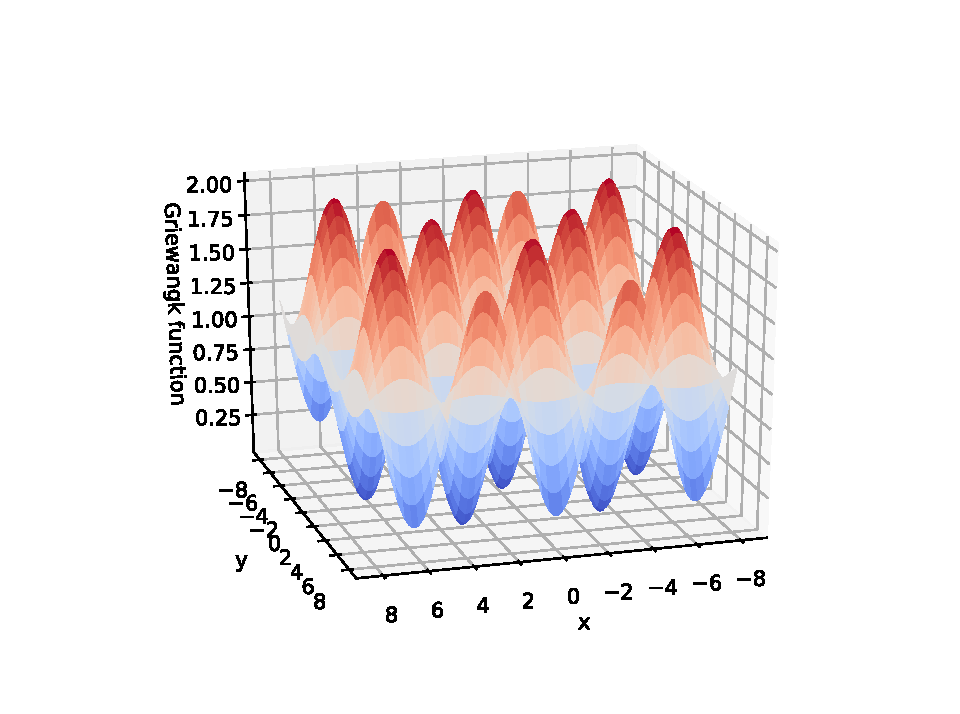
\includegraphics[width = 300pt]{svg/Griewangk2_svg-tex.pdf}
  \caption{Griewangk function only in the interval [-8,8]}
\end{figure}
%\end{comment}
\subsubsection{Rastrigin function}
Rastrigin function has the following definition:
$$f(x) = 10 \cdot n + \sum_{i=1}^n\left(x_i^2 - 10\cdot cos(2 \cdot \pi \cdot x_i)\right), -5.12 \leq x_i \leq 5.12$$
having the global optima of: $f(x) = 0, x(i) = 0, i = 1:n$. 
%\begin{comment} % the above lines are commented
\begin{figure}[h!]
  \centering
  \includegraphics[width = 300pt]{svg/Rastrigin1_svg-tex.pdf}
  \caption{Rastrigin function on its entire definition interval}
\end{figure}
%\end{comment}
\subsubsection{Rosenbrock function}
The Rosenbrock function is the following:
$$f(x) = \sum_{i=1}^{n-1}100\cdot\left(x_{i+1} - x_i^2\right)^2 + \left(1 - x_i\right)^2, -2.048 \leq x_i \leq 2.048$$
with the global optima $f(x) = 0, x(i) = 1, i = 1:n$.
%\begin{comment} % the above lines are commented
\begin{figure}[h!]
  \centering
  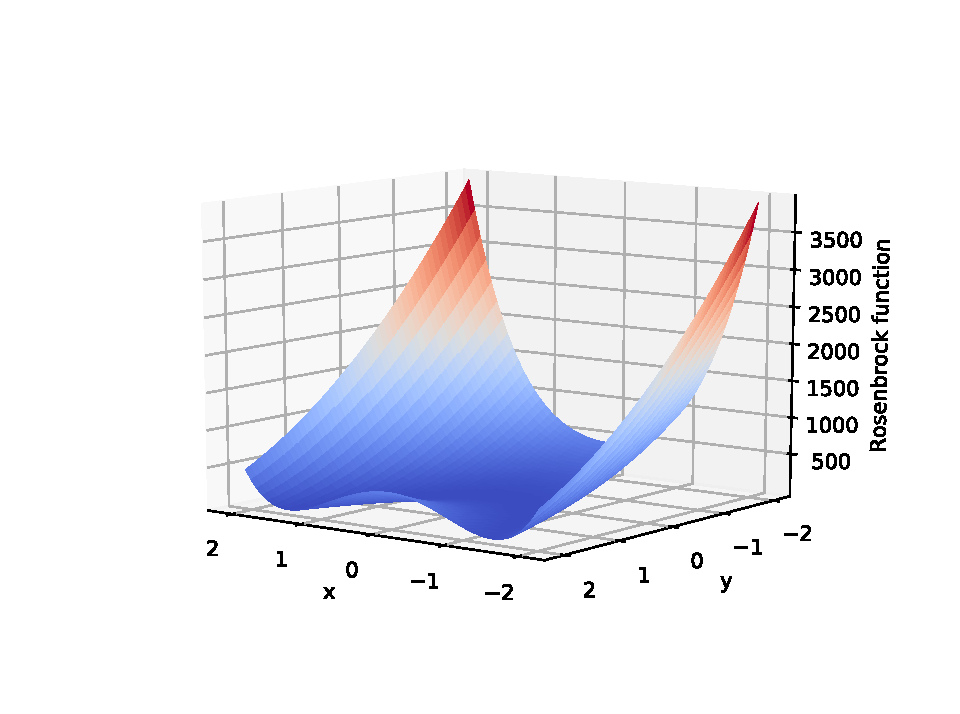
\includegraphics[width = 300pt]{svg/Rosenbrock_svg-tex.pdf}
  \caption{Rosenbrock function on its entire definition interval}
\end{figure}
%\end{comment}
\subsubsection{Six-hump Camelback}
The Six-hump Camelback has the following definition:
$$f(x) = \left(4 - 2.1 \cdot x_1^2 + \frac{x_1^4}{3}\right) \cdot x_1 ^2 + x_1 \cdot x_2 + \left(-4 + 4 \cdot x_2^2\right) \cdot x_2^2,$$ $$-3 \leq x_1 \leq 3, -2 \leq x_2 \leq 2$$
and its global optima is $$f(x_1, x_2) = -1.0316, (x_1, x_2) = (-0.0898,0.7126), (0.0898,-0.7126).$$
%\begin{comment} % the above lines are commented
\begin{figure}[h!]
  \centering
  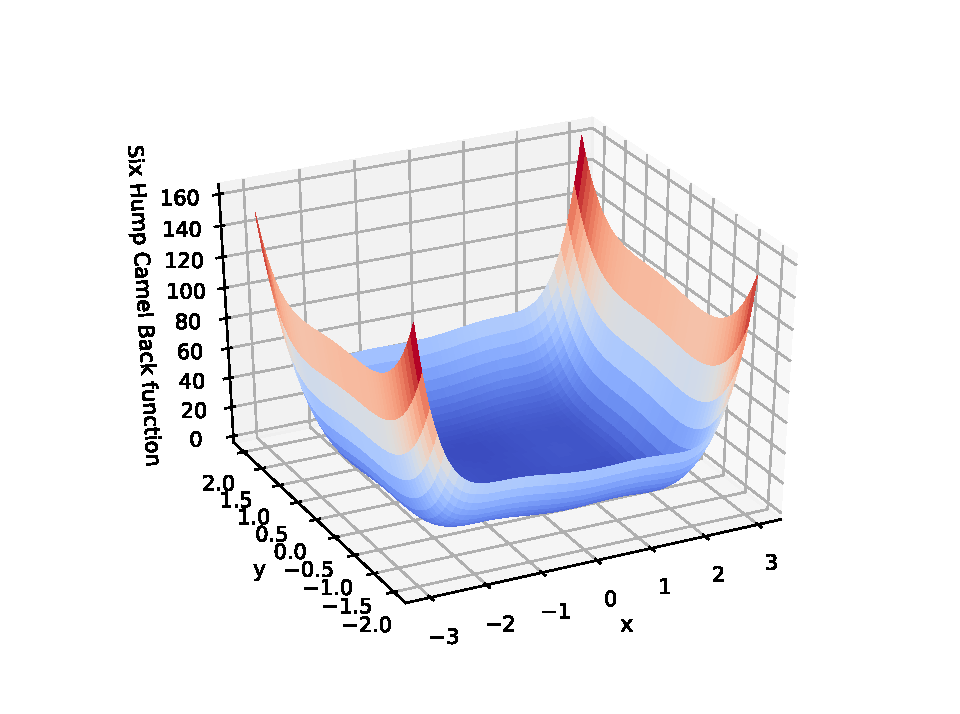
\includegraphics[width = 300pt]{svg/Sixhumpcamelback_svg-tex.pdf}
  \caption{Six-hump Camelback function on its entire definition interval}
\end{figure}
%\end{comment}


\section{Experiments}

Some of the experiments we have tried as part of the optimization problem.

\begin{enumerate} 
	\item Genetic algorithm
	\begin{enumerate}
		\item \label{experiment:1a} Low crossover probability: 
		\begin{itemize}
			\item crossover probability: 0.1
			\item bit mutation probability: 0.01
			\item chromosome mutation probability: 0.1
			\item selection: roulette
		\end{itemize} 
		\item \label{experiment:1b} High crossover probability:
		\begin{itemize}
			\item crossover probability: 0.6
			\item bit mutation probability: 0.01
			\item chromosome mutation probability: 0.1
			\item selection: roulette
		\end{itemize}
	\end{enumerate} 
	
	\item Hill Climbing
	\begin{enumerate}
		\item \label{experiment:2a} best improvement
		\item \label{experiment:2b} first improvement
	\end{enumerate}
	
	\item Hybrid Hill Climbing
	\begin{enumerate}
		\item \label{experiment:3a} \ref{experiment:1a} with \ref{experiment:2a}
	\end{enumerate}
	
\end{enumerate}

\section{Results}

\subsection{Griewangk}

\begin{figure}[!htbp]
	\begin{tabular}{||c|||l|l|l||}
		\hline
		Experiment & Min & Max & Mean \\ \hline \hline
		\ref{experiment:1a} & 11.26 & 28.92 & 17.30 \\ \hline
		\ref{experiment:1b} & 12.33 & 29.62 & 19.89 \\ \hline
		\ref{experiment:2a} & 2.56-09 & 2.56-09 & 2.56-09 \\ \hline
		\ref{experiment:2b} & 0.03 & 2.56-09 & 0.40 \\ \hline
		\ref{experiment:3a} & 0.001 & 2.56-09 & 0.04 \\ \hline
	\end{tabular}
	\caption{minimum, maximum and the mean values for each experiment}
\end{figure}
\FloatBarrier

\subsubsection{Genetic Algorithm}
\begin{figure}[!htbp]
	\centering
	\begin{minipage}{.48\textwidth}
		\centering
		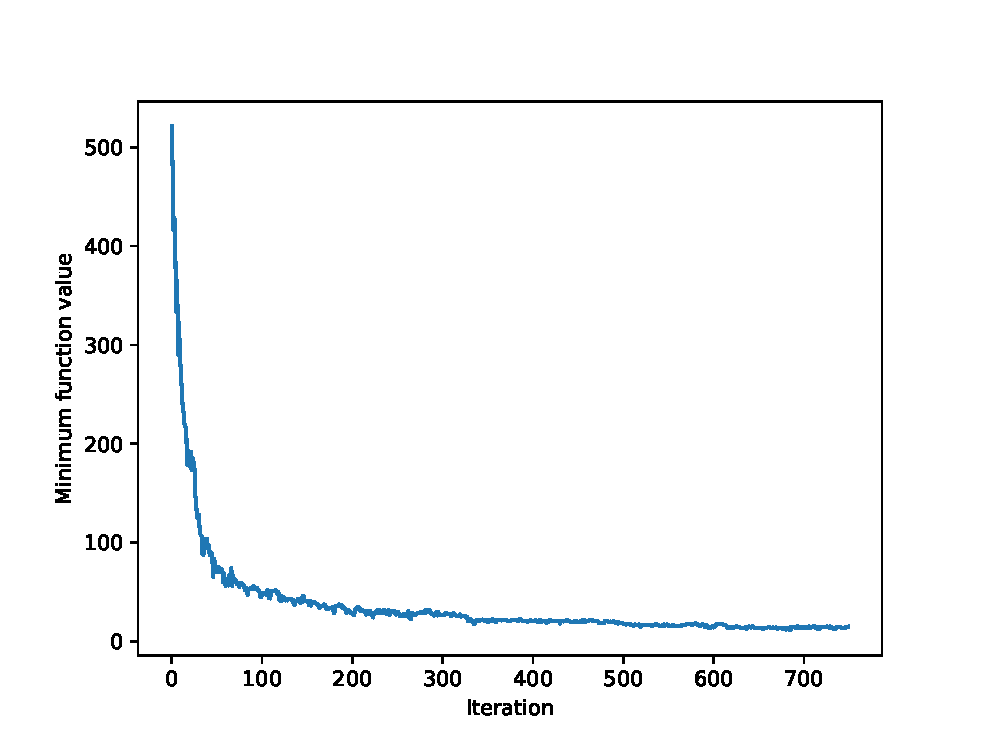
\includegraphics[scale=.4]{experiment_1a_griewangk/min_eval_0.eps}
		\caption{Function value - \ref{experiment:1a}}
	\end{minipage}\hfill
	\begin{minipage}{.48\textwidth}
		\centering
		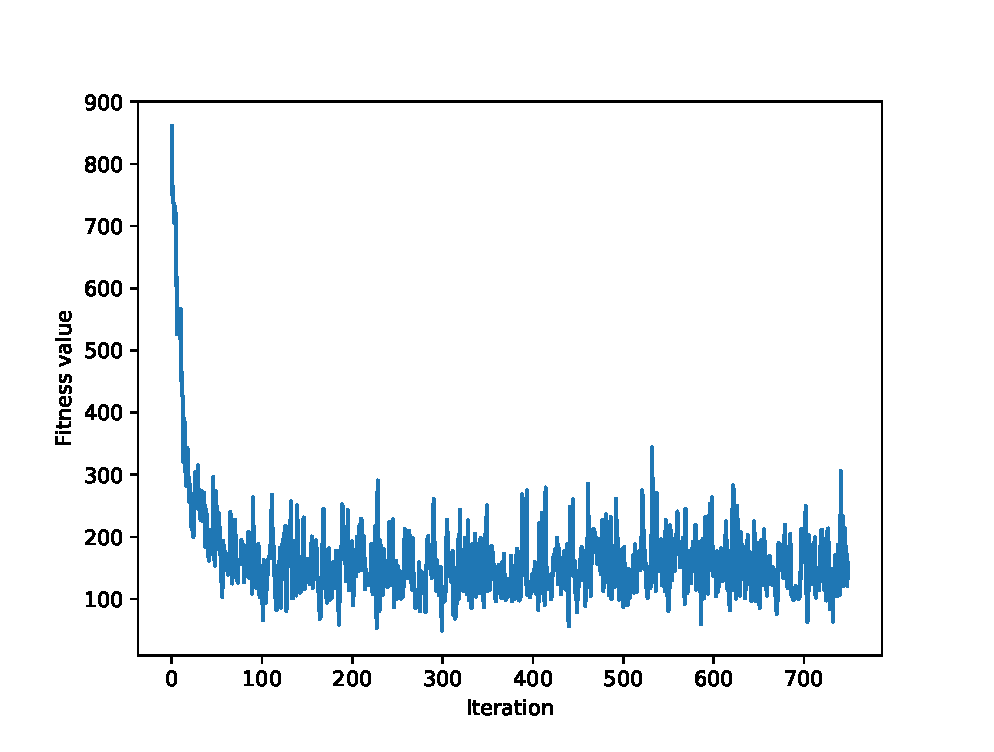
\includegraphics[scale=.4]{experiment_1a_griewangk/max_fitness_0.eps}
		\caption{Fitness value- \ref{experiment:1a}}
	\end{minipage}
\end{figure}

\FloatBarrier

\begin{figure}[!htbp]
	\centering
	\begin{minipage}{.48\textwidth}
		\centering
		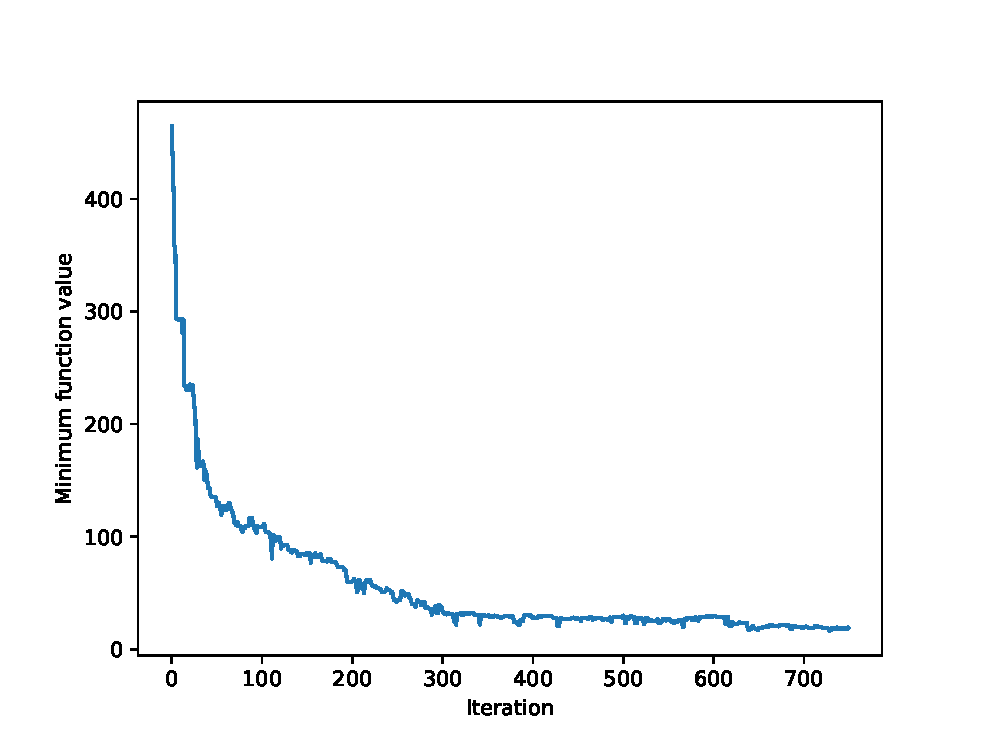
\includegraphics[scale=.4]{experiment_1b_griewangk/min_eval_0.eps}
		\caption{Function value - \ref{experiment:1b}}
	\end{minipage}\hfill
	\begin{minipage}{.48\textwidth}
		\centering
		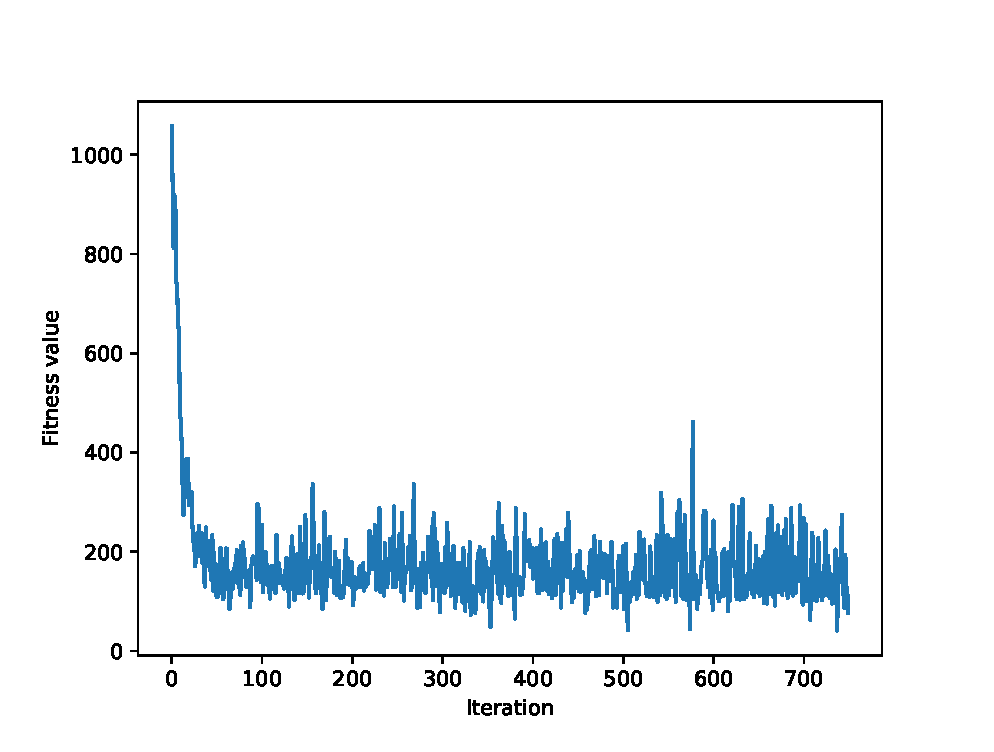
\includegraphics[scale=.4]{experiment_1b_griewangk/max_fitness_0.eps}
		\caption{Fitness value - \ref{experiment:1b}}
	\end{minipage}
\end{figure}
\FloatBarrier

\subsubsection{Hill Climbing}
\begin{figure}[!htbp]
	\centering
	\begin{minipage}{.48\textwidth}
		\centering
		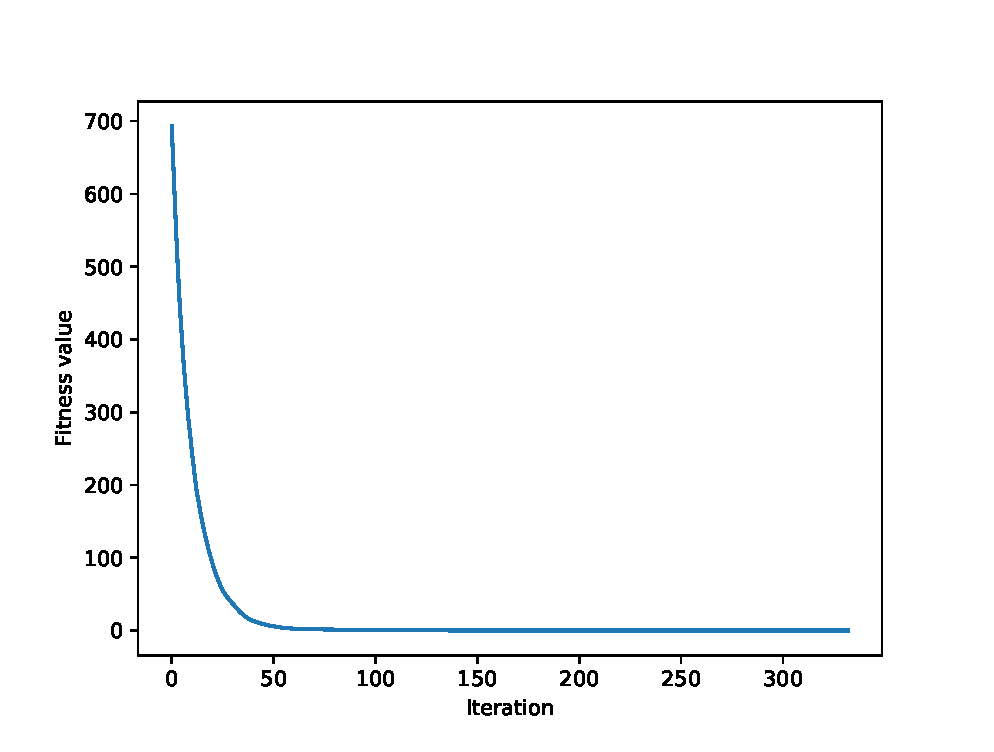
\includegraphics[scale=.4]{experiment_2a_griewangk/max_fitness_0.eps}
		\caption{Best improvement}
	\end{minipage}\hfill
	\begin{minipage}{.48\textwidth}
		\centering
		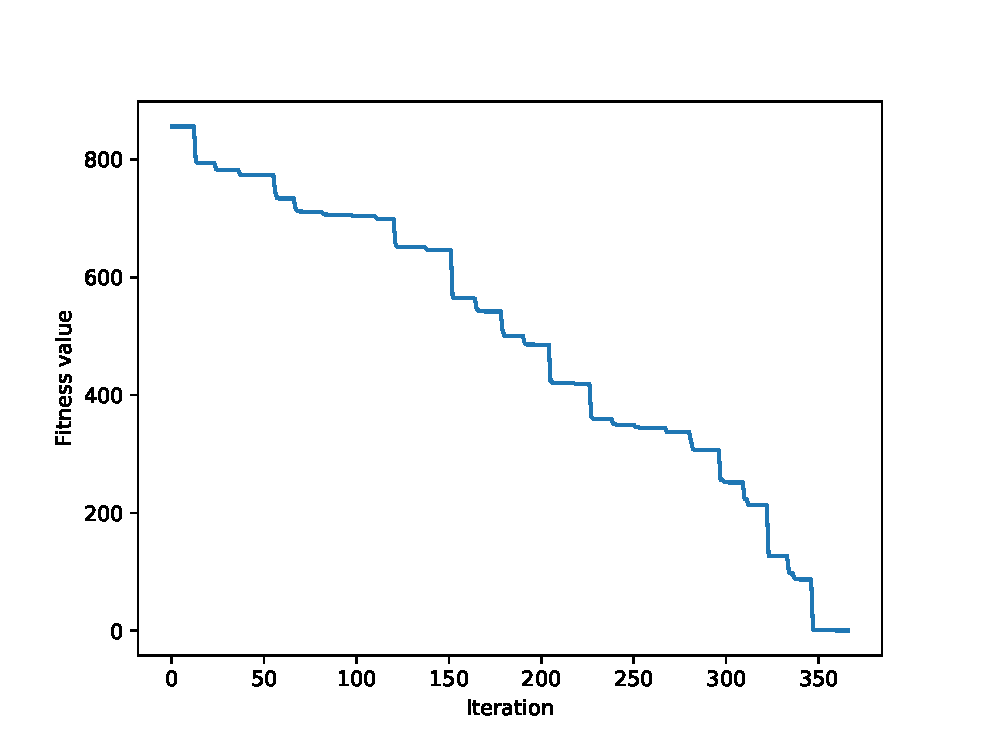
\includegraphics[scale=.4]{experiment_2b_griewangk/max_fitness_0.eps}
		\caption{First improvement}
	\end{minipage}\hfill
\end{figure}
\FloatBarrier

\subsubsection{Hybrid}
\begin{figure}[!htbp]
	\centering
	\begin{minipage}{.48\textwidth}
		\centering
		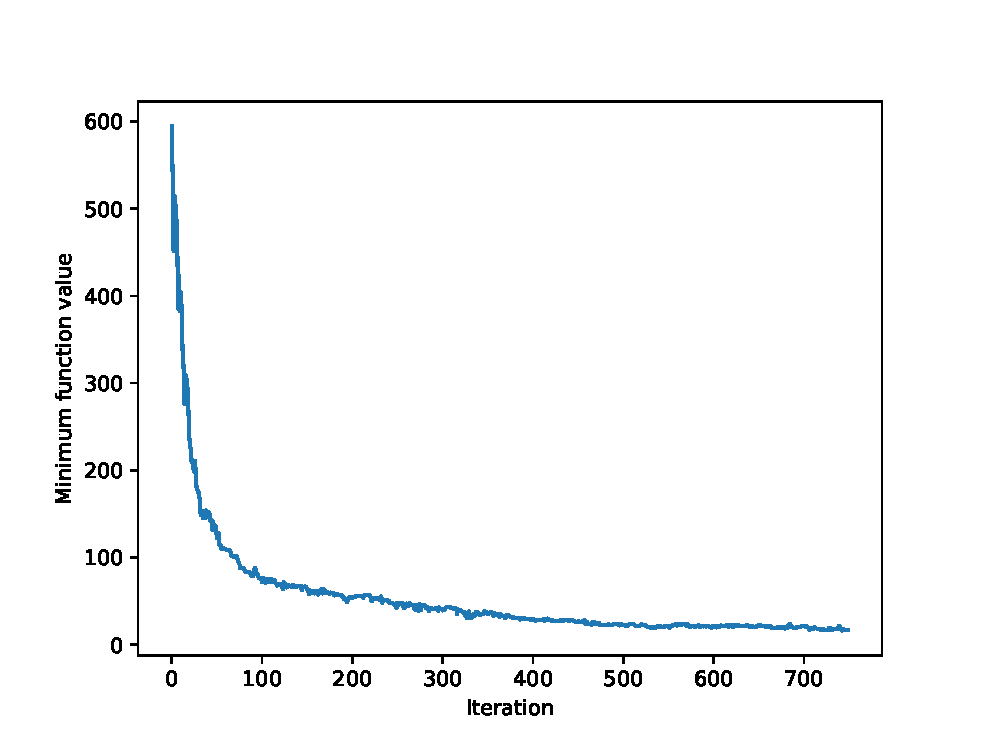
\includegraphics[scale=.4]{experiment_3a_griewangk/ga_min_eval_0.eps}
		\caption{Genetic algorithm}
	\end{minipage}\hfill
	\begin{minipage}{.48\textwidth}
		\centering
		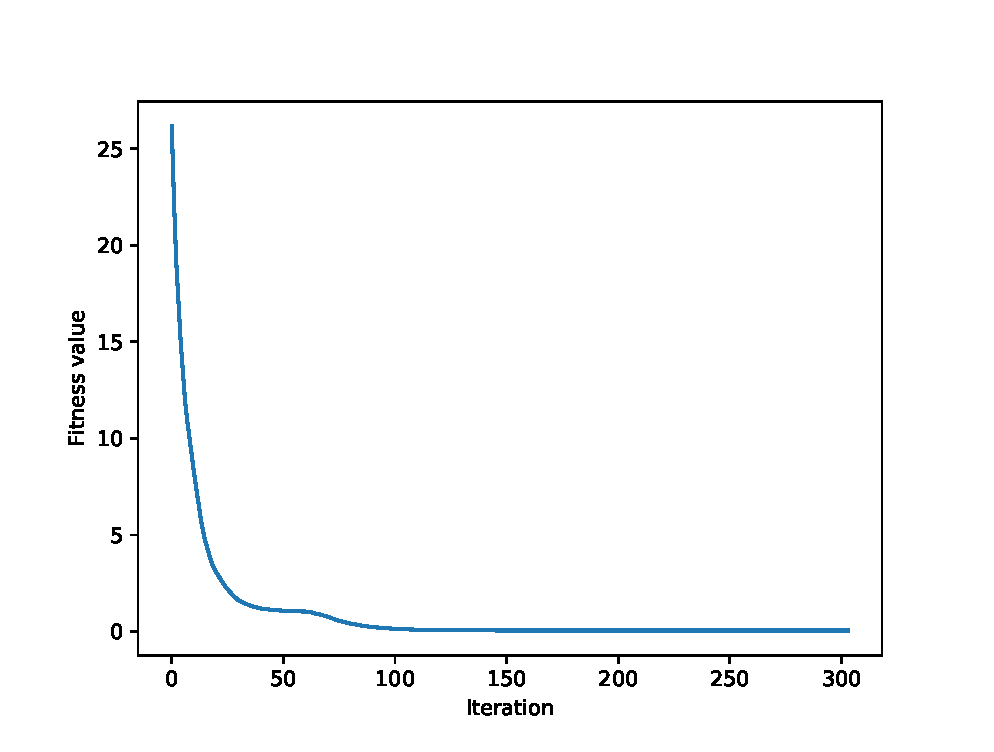
\includegraphics[scale=.4]{experiment_3a_griewangk/hc_max_fitness_0.eps}
		\caption{Hill Climbing}
	\end{minipage}\hfill
\end{figure}
\FloatBarrier

\subsubsection{Interpretation}
\begin{figure}[!htbp]
	\centering
	\begin{minipage}{\textwidth}
		\centering
		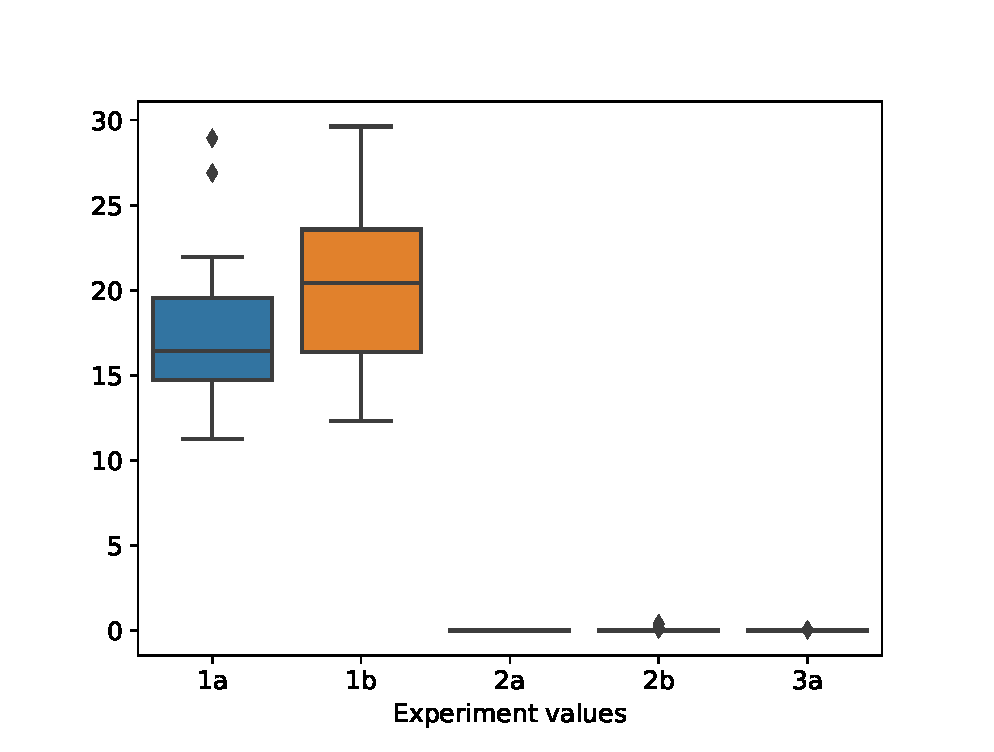
\includegraphics[scale=.8]{boxplots/griewangk_boxplot.eps}
		\caption{Griewangk experiments boxplot}
		\label{fig:griewangk_experiments_boxplot}
	\end{minipage}\hfill
\end{figure}
\FloatBarrier

\begin{figure}[!htbp]
	\centering
	\begin{minipage}{\textwidth}
		\centering
		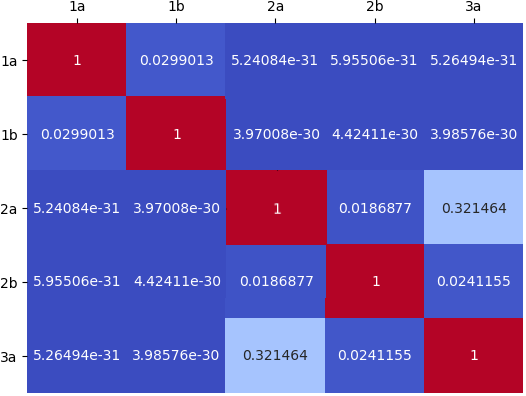
\includegraphics[scale=.8]{t_test/griewangk_t_test_matrix.png}
		\caption{Griewangk experiments t test matrix}
		\label{fig:griewangk_experiments_t_test}
	\end{minipage}\hfill
\end{figure}
\FloatBarrier
\paragraph{Observations} We can observe in Fig. \ref{fig:griewangk_experiments_boxplot} that the experiments \ref{experiment:1a} and \ref{experiment:1b} have the worst results but we can't really say which of the other three is the best. The t test does not give a significant p value to affirm that the experiments means differ.

\subsection{Rastrigin}

\begin{figure}[!htbp]
	\begin{tabular}{||c|||l|l|l||}
		\hline
		Experiment & Min & Max & Mean \\ \hline \hline
		\ref{experiment:1a} & 44.09 & 85.05 & 64.57  \\ \hline
		\ref{experiment:1b} & 50.77 & 107.90 & 76.33 \\ \hline
		\ref{experiment:2a} & 26.78 & 59.28 & 44.77  \\ \hline
		\ref{experiment:2b} & 50.97 & 76.22 & 57.91  \\ \hline
		\ref{experiment:3a} & 24.30 & 39.43 & 32.16  \\ \hline
	\end{tabular}
	\caption{minimum, maximum and the mean values for each experiment}
\end{figure}
\FloatBarrier

\subsubsection{Genetic Algorithm}
\begin{figure}[!htbp]
	\centering
	\begin{minipage}{.48\textwidth}
		\centering
		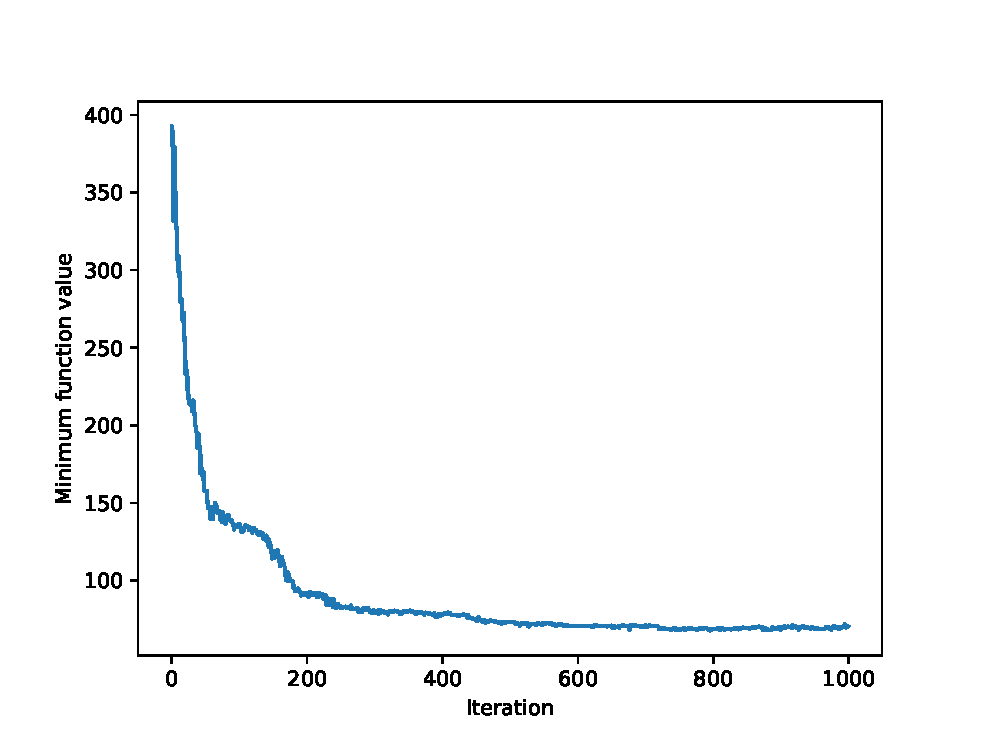
\includegraphics[scale=.4]{experiment_1a_rastrigin/min_eval_0.eps}
		\caption{Function value - \ref{experiment:1a}}
	\end{minipage}\hfill
	\begin{minipage}{.48\textwidth}
		\centering
		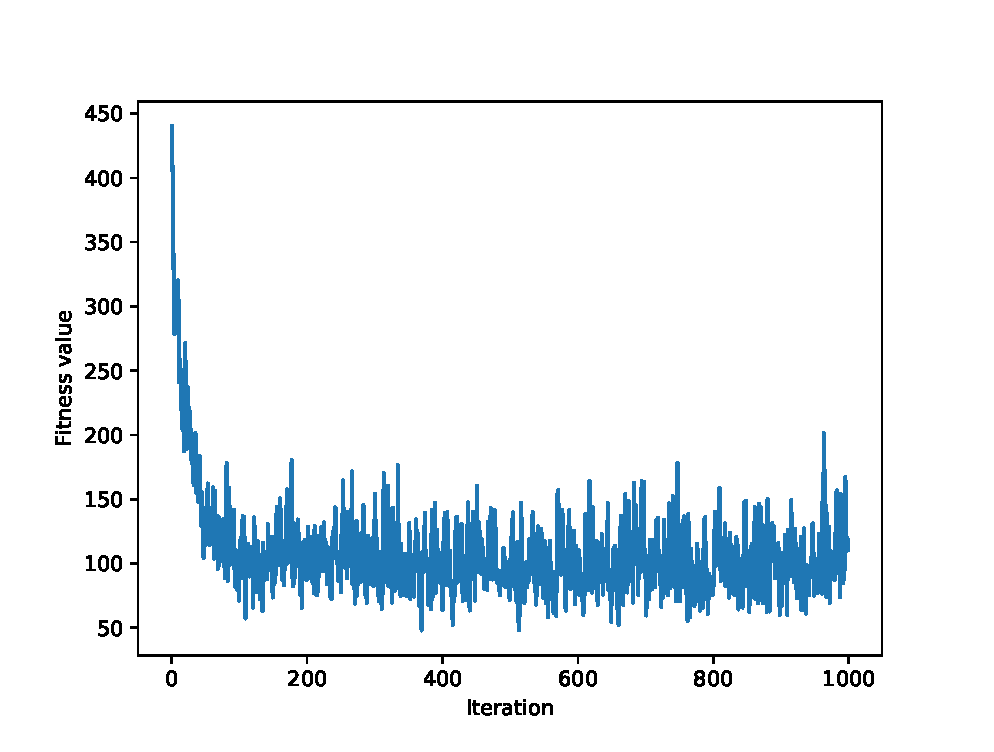
\includegraphics[scale=.4]{experiment_1a_rastrigin/max_fitness_0.eps}
		\caption{Fitness value - \ref{experiment:1a}}
	\end{minipage}
\end{figure}
\FloatBarrier

\begin{figure}[!htbp]
	\centering
	\begin{minipage}{.48\textwidth}
		\centering
		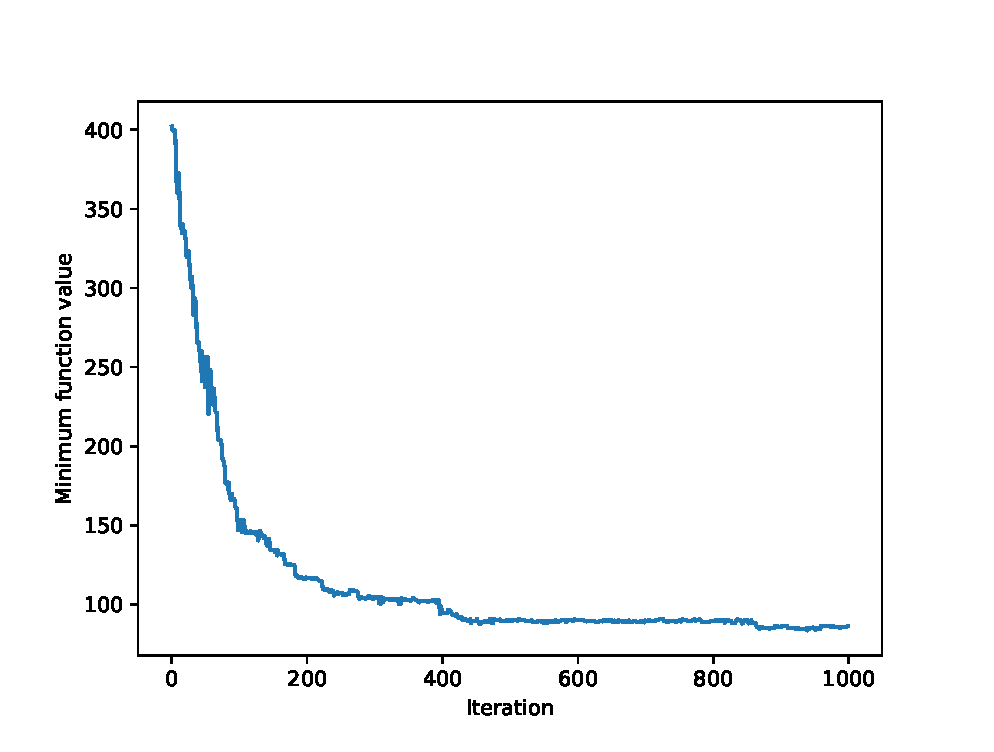
\includegraphics[scale=.4]{experiment_1b_rastrigin/min_eval_0.eps}
		\caption{Function value - \ref{experiment:1b}}
	\end{minipage}\hfill
	\begin{minipage}{.48\textwidth}
		\centering
		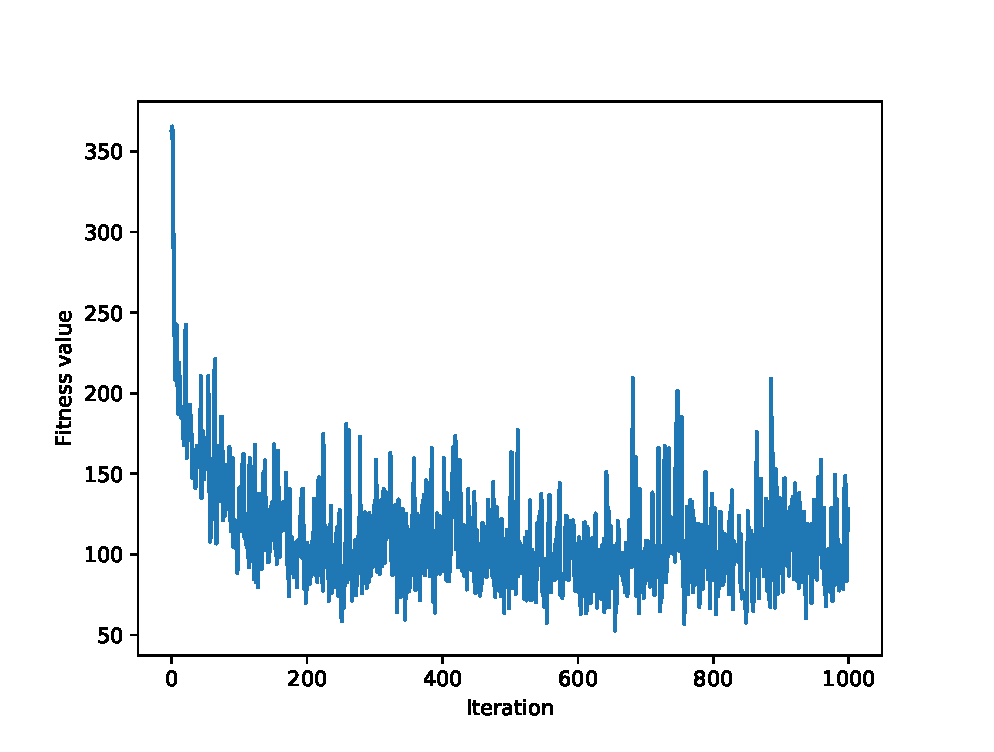
\includegraphics[scale=.4]{experiment_1b_rastrigin/max_fitness_0.eps}
		\caption{Fitness value - \ref{experiment:1b}}
	\end{minipage}
\end{figure}
\FloatBarrier
\subsubsection{Hill Climbing}
\begin{figure}[!htbp]
	\centering
	\begin{minipage}{.48\textwidth}
		\centering
		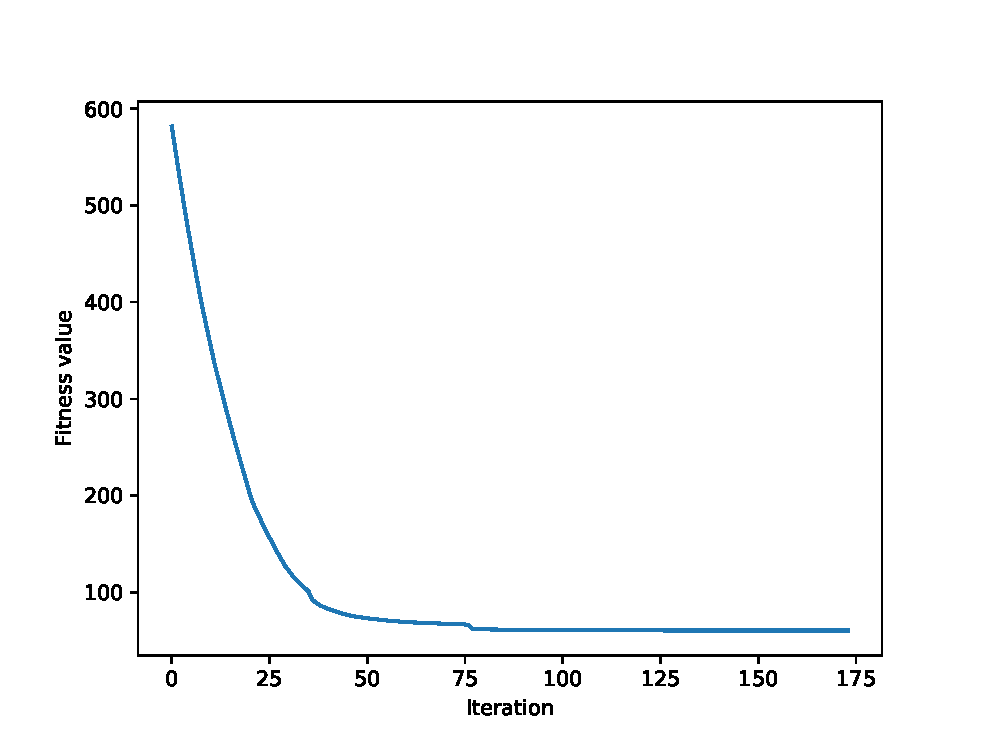
\includegraphics[scale=.4]{experiment_2a_rastrigin/max_fitness_0.eps}
		\caption{Best improvement}
	\end{minipage}\hfill
	\begin{minipage}{.48\textwidth}
		\centering
		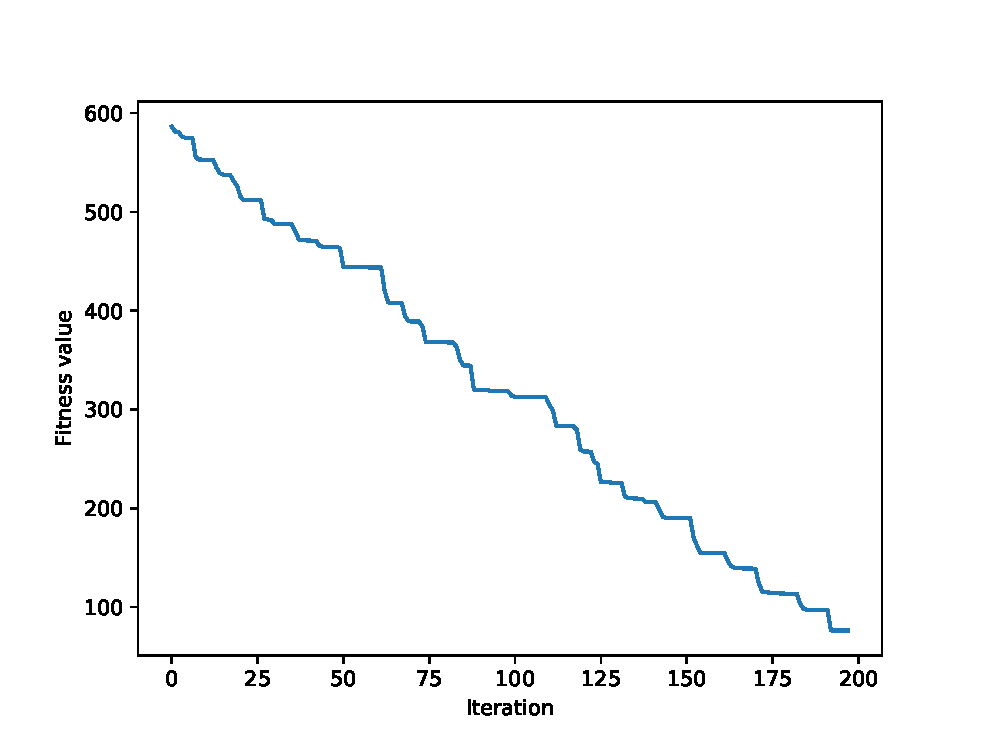
\includegraphics[scale=.4]{experiment_2b_rastrigin/max_fitness_0.eps}
		\caption{First improvement}
	\end{minipage}\hfill
\end{figure}
\FloatBarrier

\subsubsection{Hybrid}
\begin{figure}[!htbp]
	\centering
	\begin{minipage}{.48\textwidth}
		\centering
		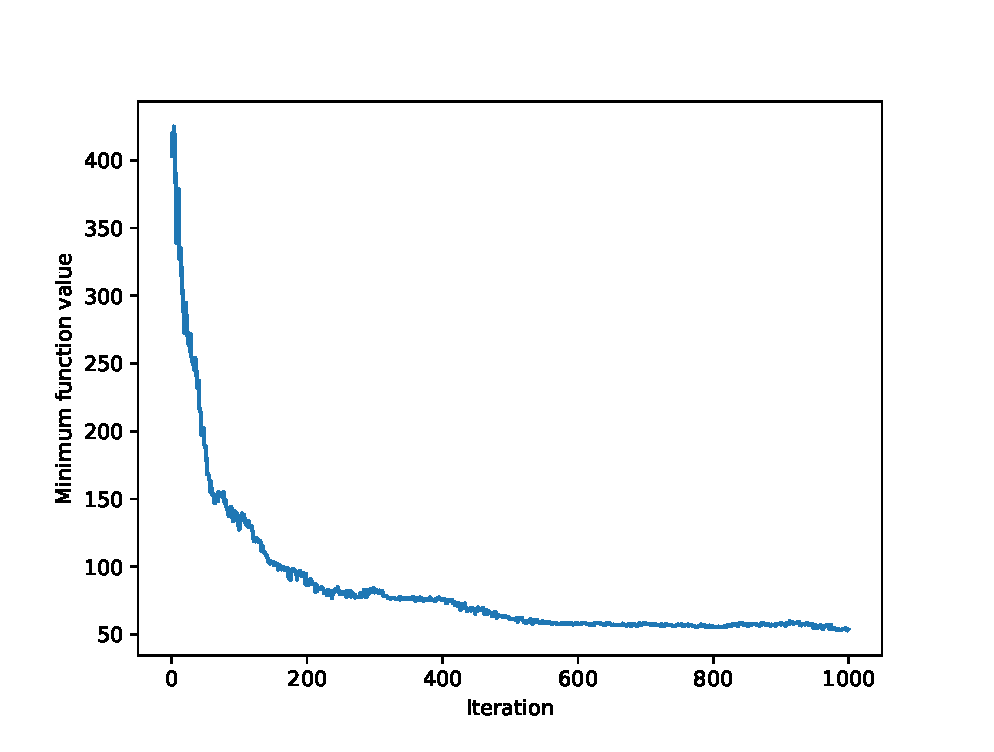
\includegraphics[scale=.4]{experiment_3a_rastrigin/ga_min_eval_0.eps}
		\caption{Genetic algorithm}
	\end{minipage}\hfill
	\begin{minipage}{.48\textwidth}
		\centering
		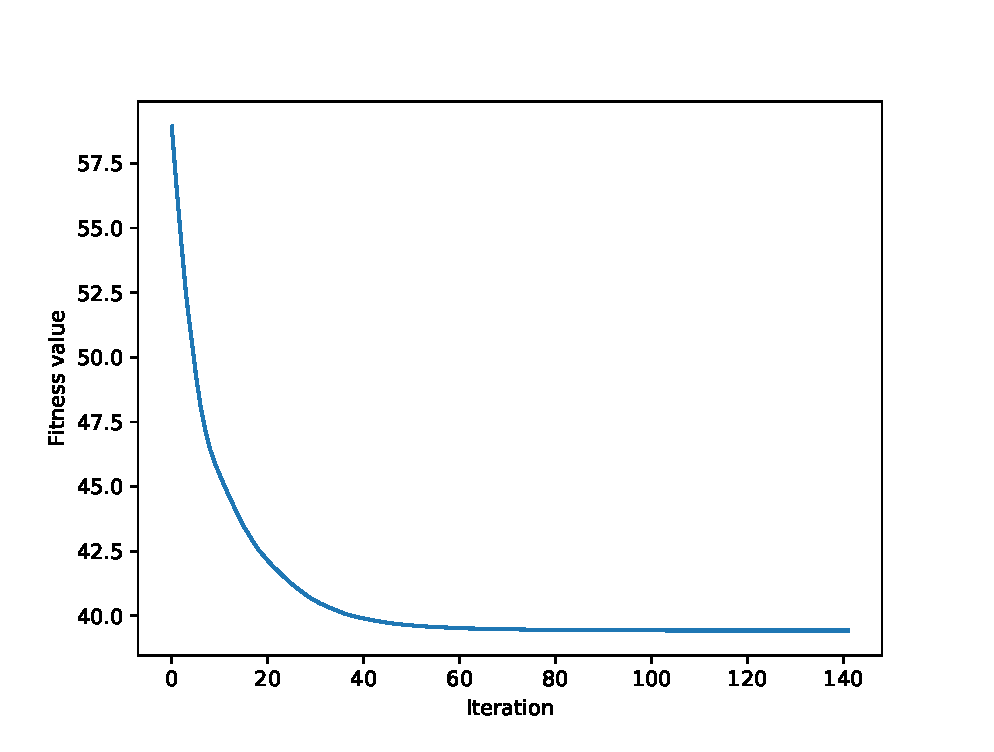
\includegraphics[scale=.4]{experiment_3a_rastrigin/hc_max_fitness_0.eps}
		\caption{Hill Climbing}
	\end{minipage}\hfill
\end{figure}
\FloatBarrier

\subsubsection{Interpretation}
\begin{figure}[!htbp]
	\centering
	\begin{minipage}{\textwidth}
		\centering
		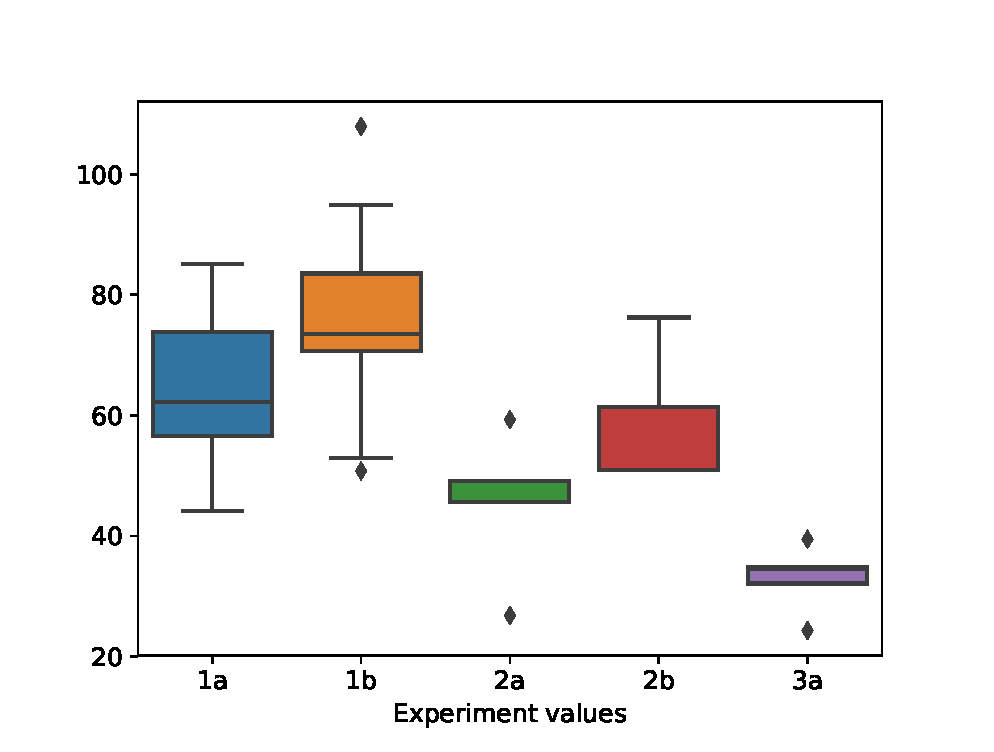
\includegraphics[scale=.8]{boxplots/rastrigin_boxplot.eps}
		\caption{Rastrigin experiments boxplot}
		\label{fig:rastrigin_experiments_boxplot}
	\end{minipage}\hfill
\end{figure}
\FloatBarrier

\begin{figure}[!htbp]
	\centering
	\begin{minipage}{\textwidth}
		\centering
		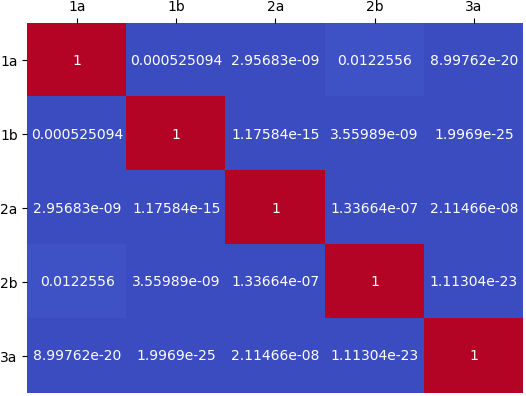
\includegraphics[scale=.8]{t_test/rastrigin_t_test_matrix.png}
		\caption{Rastrigin experiments t test matrix}
		\label{fig:rastrigin_experiments_t_test}
	\end{minipage}\hfill
\end{figure}
\FloatBarrier

\paragraph{Observations} We can observe in Fig. \ref{fig:rastrigin_experiments_boxplot} that the experiment \ref{experiment:3a} goes to the best minimum value. This conclusion is also verified using t test. We can see that in Fig. \ref{fig:rastrigin_experiments_t_test} which shows the p value between experiments.

\subsection{Rosenbrock}

\begin{figure}[!htbp]
	\begin{tabular}{||c|||l|l|l||}
		\hline
		Experiment & Min & Max & Mean \\ \hline \hline
		\ref{experiment:1a} & 154.07 & 398.18 & 253.27 \\ \hline
		\ref{experiment:1b} & 109.52 & 382.73 & 272.65 \\ \hline
		\ref{experiment:2a} & 28.13 & 122.93 & 37.68   \\ \hline
		\ref{experiment:2b} & 25.25 & 132.46 & 33.21   \\ \hline
		\ref{experiment:3a} & 23.09 & 136.88 & 26.88  \\ \hline
	\end{tabular}
	\caption{minimum, maximum and the mean values for each experiment}
\end{figure}
\FloatBarrier

\subsubsection{Genetic Algorithm}
\begin{figure}[!htbp]
	\centering
	\begin{minipage}{.48\textwidth}
		\centering
		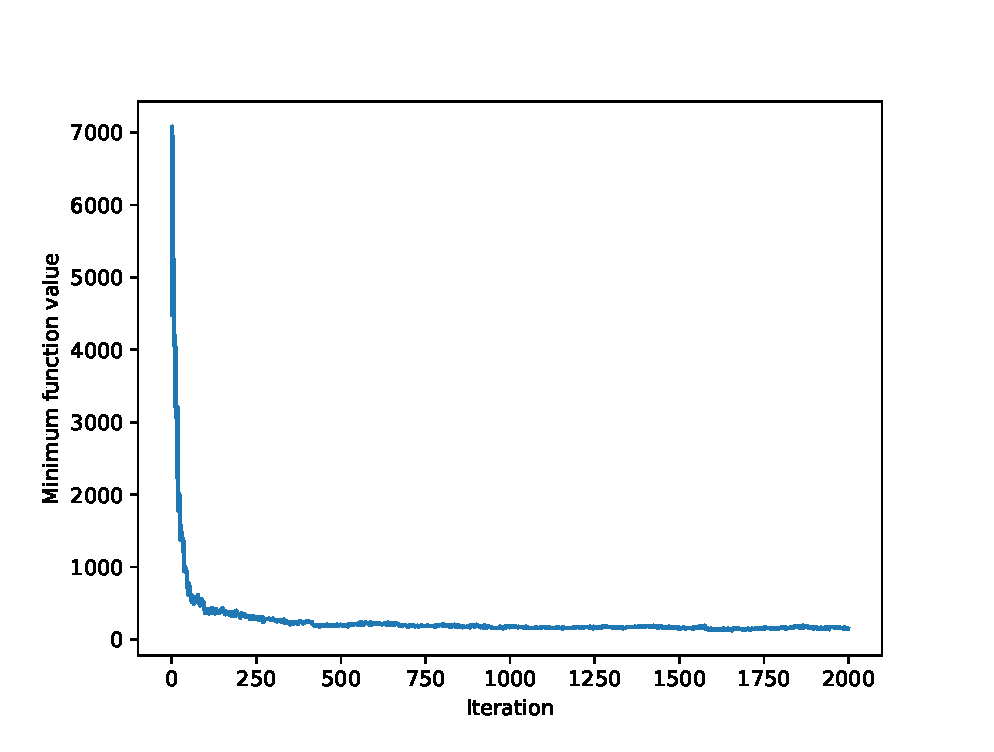
\includegraphics[scale=.4]{experiment_1a_rosenbrock/min_eval_0.eps}
		\caption{Function value - \ref{experiment:1a}}
	\end{minipage}\hfill
	\begin{minipage}{.48\textwidth}
		\centering
		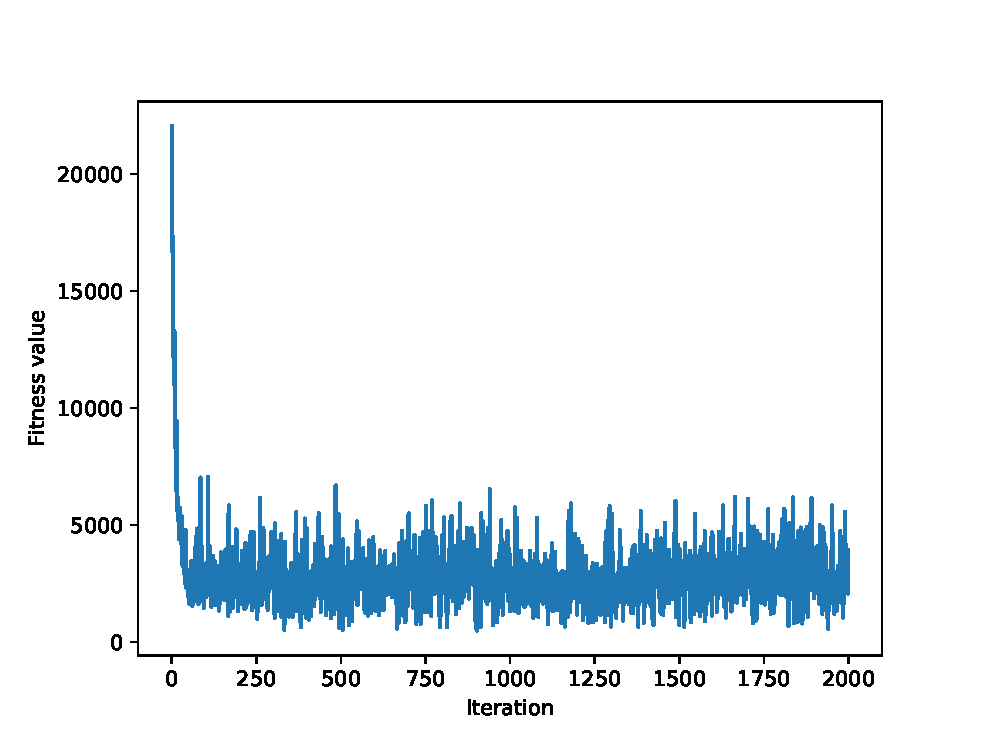
\includegraphics[scale=.4]{experiment_1a_rosenbrock/max_fitness_0.eps}
		\caption{Fitness value - \ref{experiment:1a}}
	\end{minipage}
\end{figure}
\FloatBarrier

\begin{figure}[!htbp]
	\centering
	\begin{minipage}{.48\textwidth}
		\centering
		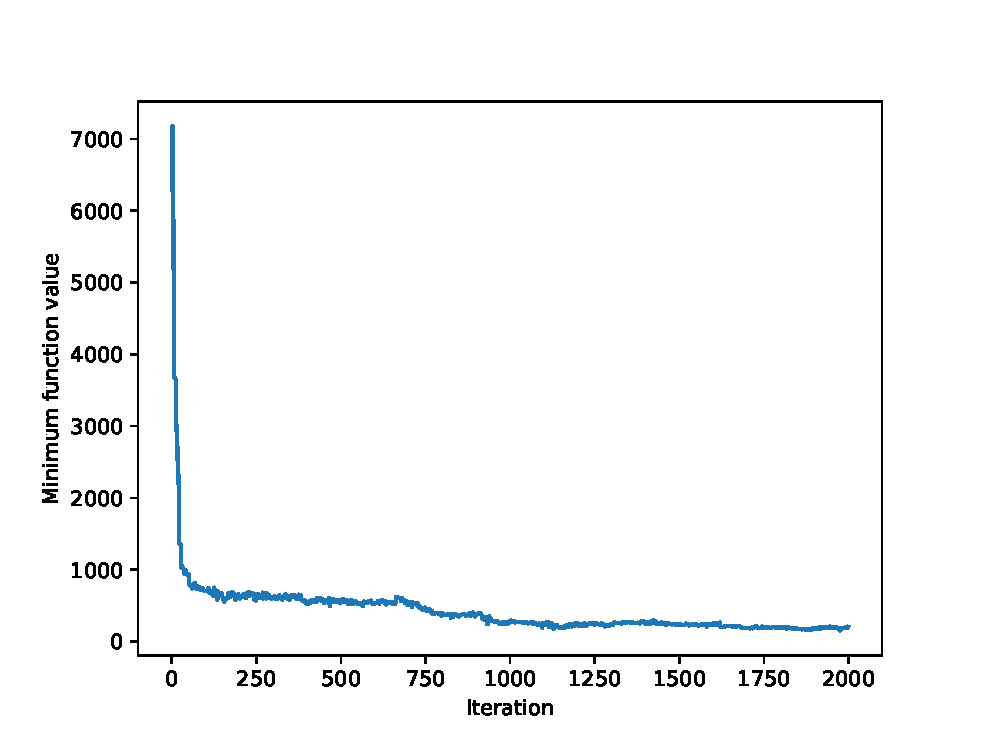
\includegraphics[scale=.4]{experiment_1b_rosenbrock/min_eval_0.eps}
		\caption{Function value - \ref{experiment:1b}}
	\end{minipage}\hfill
	\begin{minipage}{.48\textwidth}
		\centering
		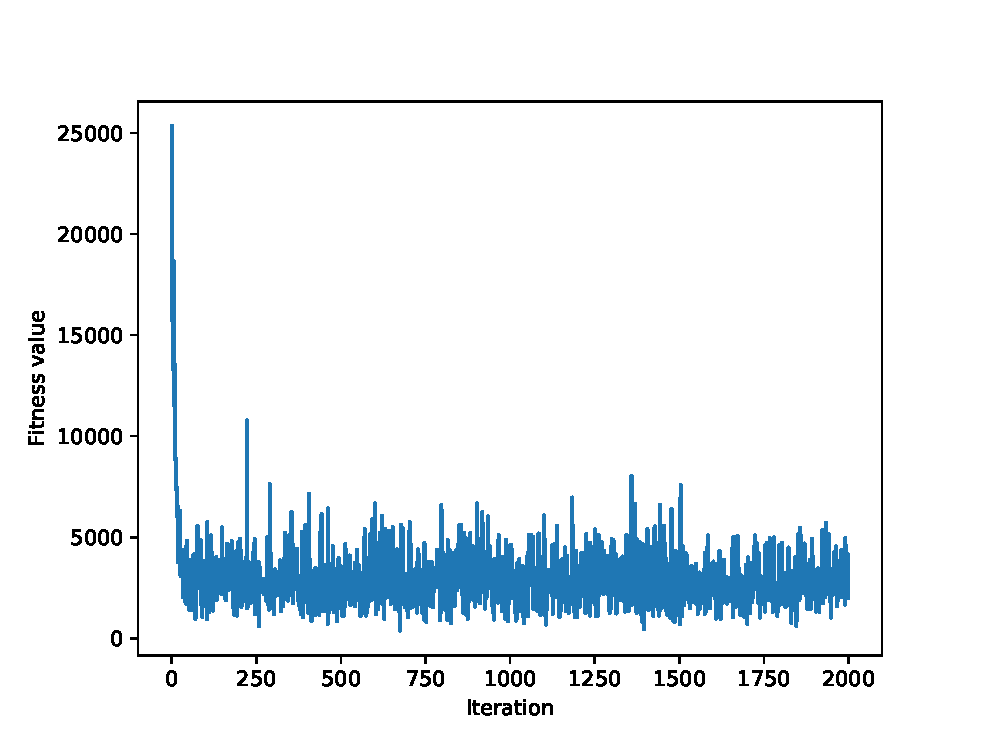
\includegraphics[scale=.4]{experiment_1b_rosenbrock/max_fitness_0.eps}
		\caption{Fitness value - \ref{experiment:1b}}
	\end{minipage}
\end{figure}
\FloatBarrier

\subsubsection{Hill Climbing}
\begin{figure}[!htbp]
	\centering
	\begin{minipage}{.48\textwidth}
		\centering
		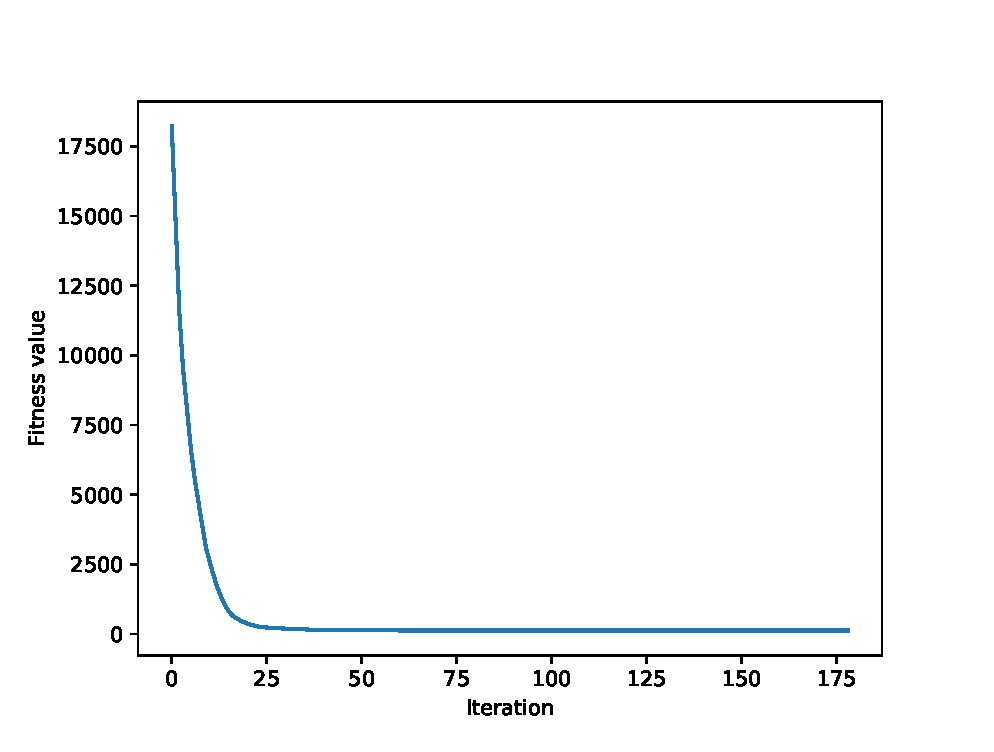
\includegraphics[scale=.4]{experiment_2a_rosenbrock/max_fitness_0.eps}
		\caption{Best improvement}
	\end{minipage}\hfill
	\begin{minipage}{.48\textwidth}
		\centering
		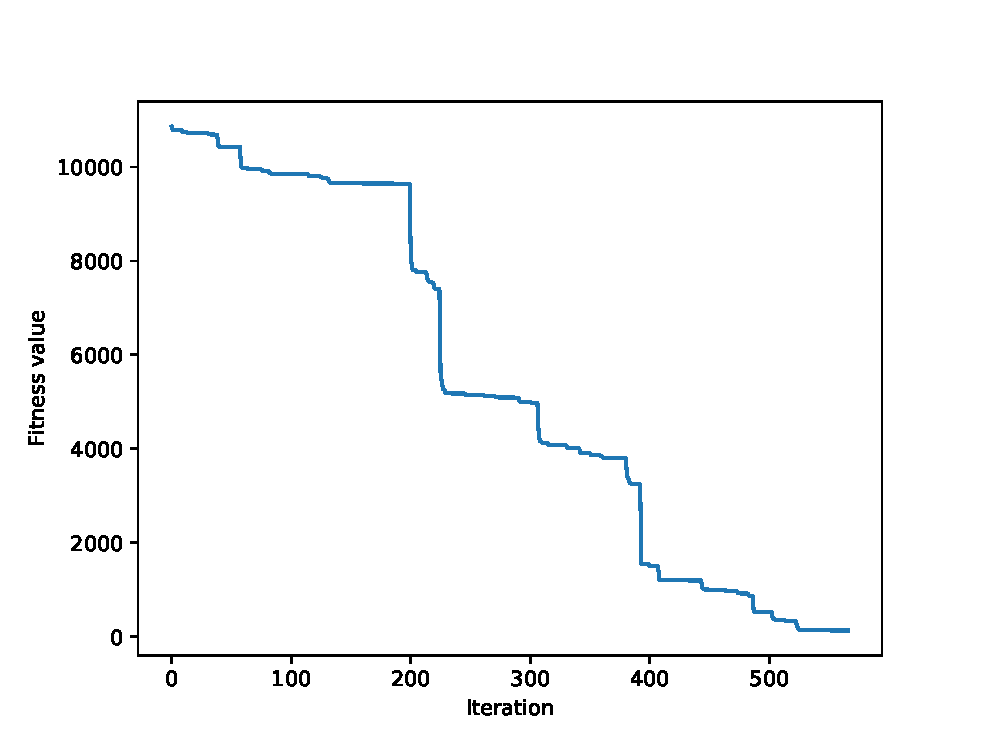
\includegraphics[scale=.4]{experiment_2b_rosenbrock/max_fitness_0.eps}
		\caption{First improvement}
	\end{minipage}\hfill
\end{figure}
\FloatBarrier

\subsubsection{Hybrid}
\begin{figure}[!htbp]
	\centering
	\begin{minipage}{.48\textwidth}
		\centering
		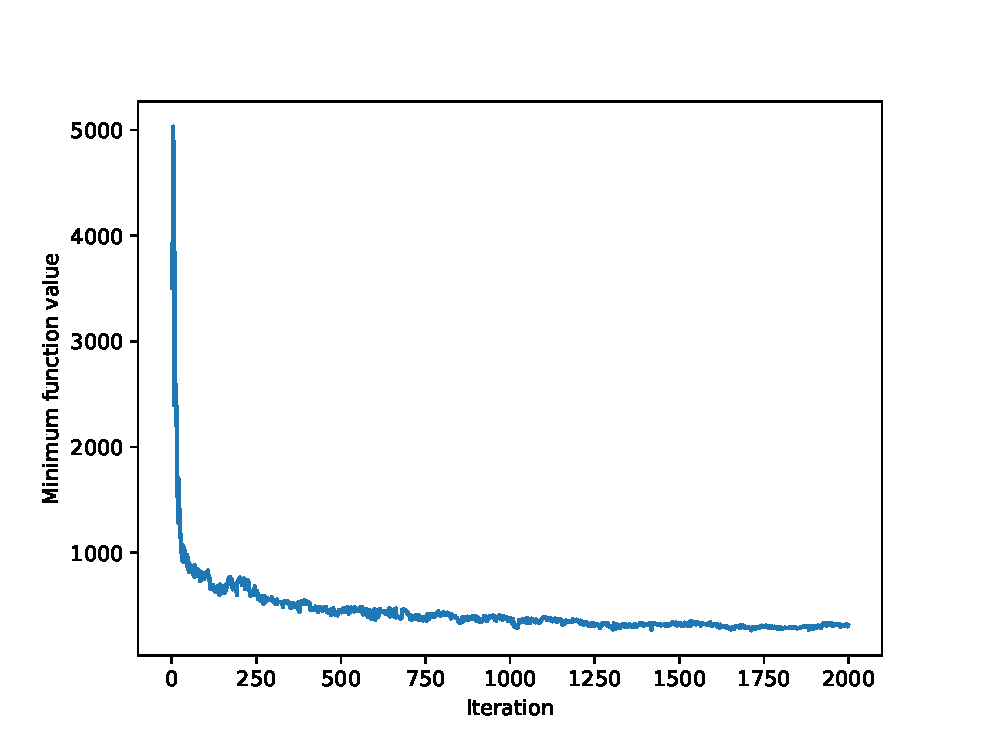
\includegraphics[scale=.4]{experiment_3a_rosenbrock/ga_min_eval_0.eps}
		\caption{Genetic algorithm}
	\end{minipage}\hfill
	\begin{minipage}{.48\textwidth}
		\centering
		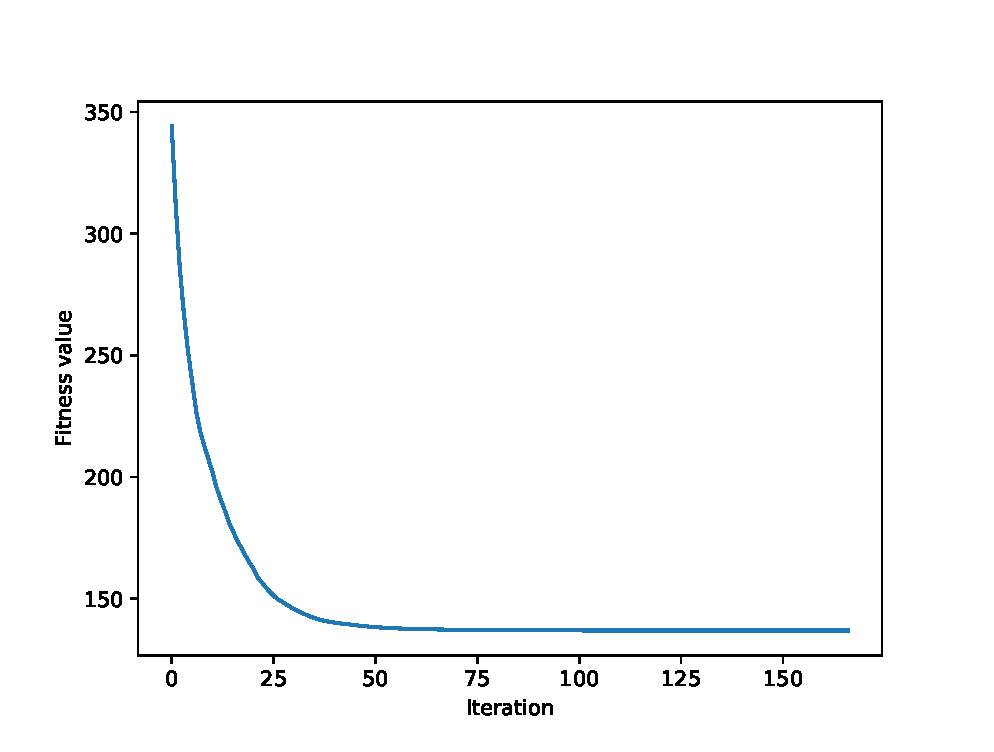
\includegraphics[scale=.4]{experiment_3a_rosenbrock/hc_max_fitness_0.eps}
		\caption{Hill Climbing}
	\end{minipage}\hfill
\end{figure}
\FloatBarrier

\subsubsection{Interpretation}
\begin{figure}[!htbp]
	\centering
	\begin{minipage}{\textwidth}
		\centering
		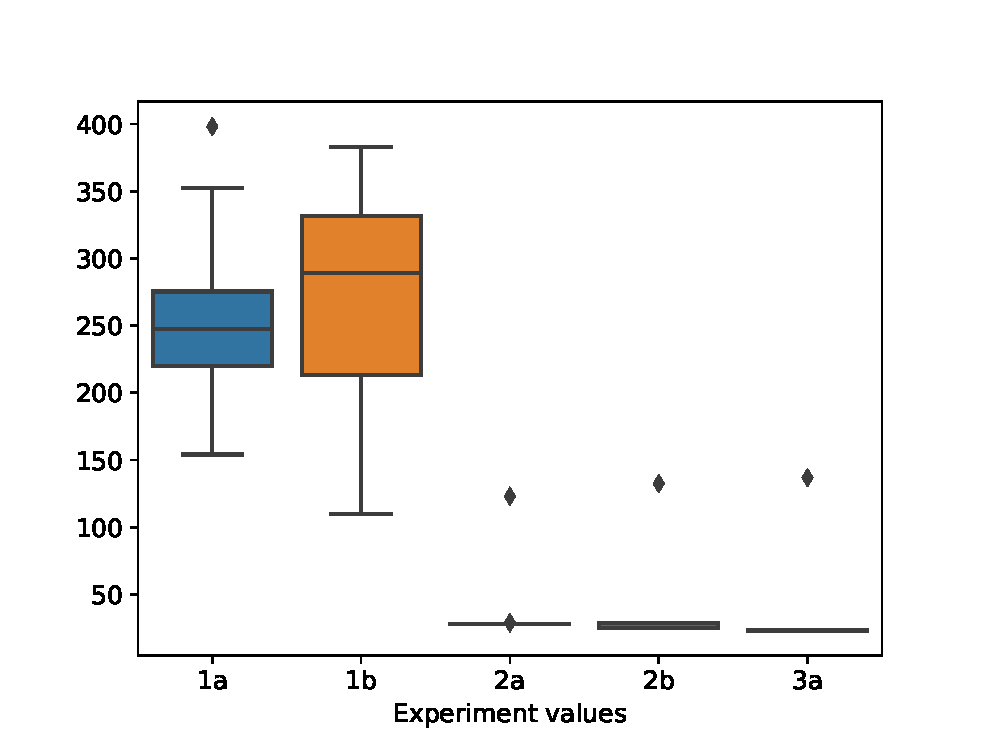
\includegraphics[scale=.8]{boxplots/rosenbrock_boxplot.eps}
		\caption{Rosenbrock experiments boxplot}
		\label{fig:rosenbrock_experiments_boxplot}
	\end{minipage}\hfill
\end{figure}
\FloatBarrier

\begin{figure}[!htbp]
	\centering
	\begin{minipage}{\textwidth}
		\centering
		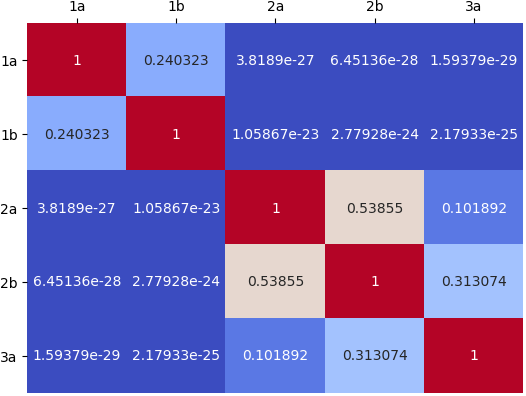
\includegraphics[scale=.8]{t_test/rosenbrock_t_test_matrix.png}
		\caption{Rosenbrock experiments t test matrix}
	\end{minipage}\hfill
\end{figure}
\FloatBarrier

\paragraph{Observations} We can observe in Fig. \ref{fig:rosenbrock_experiments_boxplot} that the experiments \ref{experiment:1a} and \ref{experiment:1b} have the worst results but we can't really say which of the other three is the best. The t test does not give a significant p value to affirm that the experiments means differ

\section{Conclusions}
\paragraph{} The results of our experiments outline the power of genetic algorithms when it comes to solving optimization problems.
\paragraph{} We have seen that Genetic Algorithm used with a fixed number of iterations (in our case it varies from 750 to 1000 depending on when we observe that the algorithm converges) did not give better results than the hill climbing algorithm. This may change if we increase the number of iterations. However, if we combine the two algorithms we obtain slightly better results.
\paragraph{} Comparing the hybrid solution with the standalone Genetic Algorithms is pretty much redundant as it's in the nature of the algorithm to give better results or at least as good as the ones provided by the GA.
 
\paragraph{} The hybrid solution also outshone the other solutions for Rastrigin function, this can be observed in the experiments above. For the other functions the results were at least as good as the ones provided by the other solutions. 

\bibliographystyle{plain}
\begin{thebibliography}{9}
\bibitem{} 
Melanie Mitchell, "An introduction to genetic algorithms", 1998
\\\url{https://www.academia.edu/12824545/An_Introduction_to_Genetic_Algorithms_-_Melanie_Mitchell}
\bibitem{} 
Breaban Mihaela, Nature Inspired Methods class course, 2020
\\\url{https://profs.info.uaic.ro/~pmihaela/MOC/trajectory.html}

\bibitem{} 
Wikipedia site for Selection, Mutation and Crossover
\\\url{https://en.wikipedia.org/wiki/Selection_(genetic_algorithm)}
\\\url{https://en.wikipedia.org/wiki/Mutation_(genetic_algorithm)}
\\\url{https://en.wikipedia.org/wiki/Crossover_(genetic_algorithm}

\bibitem{}
MIT Open Course, "A Basic Introduction to Genetic Algorithms", Prof. Olivier de Weck, 2010
\\\url{https://ocw.mit.edu/courses/institute-for-data-systems-and-society/ids-338j-multidisciplinary-system-design-optimization-spring-2010/lecture-notes/MITESD_77S10_lec11.pdf}
\end{thebibliography}
\end{document}
